\section{Grundlagen}
\label{sec:grundlagen}
In diesem Versuch werden verschiedene Schaltungen mit Hilfe des
Operationsverstärkers realisiert.
Zunächst wird auf die physikalischen Eigenschaften eingegangen,
woraufhin verschiedene Schaltungen skizziert und schließlich
realisiert werden.

\subsection{Eigenschaften des Operationsverstärkers}
\label{subsec:eigenschaften}
Die wichtigste elektrische Eigenschaft des Operationsverstärkers
ist die Proportionalität der Ausgangsspannung $U_\text{A}$ zur
Differenz der Eingangsspannungen $U_\text{p}$ und $U_\text{N}$:
\begin{equation}
\label{eq:proportionalität}
    U_\text{A} = V(U_\text{p} - U_\text{N})\,,
\end{equation}
wobei $V$ die Leerlaufverstärkung bezeichnet.
Diese Beziehung gilt in einem Spannungsbereich
$-U_\text{B} < U_\text{A} < U_\text{B}$, der durch die Betriebsspannung
$U_\text{B}$ bestimmt ist. Ausserhalb dieses Bereichs läuft die
Ausgangsspannung in eine Sättigung.
Die Eingangsspannung $U_\text{p}$ wird nicht invertiert, während die Spannung
$U_\text{N}$ invertiert wird -- der Verstärker besitzt also einen
nicht-invertierenden und einen invertierenden Eingang.

Aus technischer Sicht entspricht der Operationsverstärker einem
gleichstromgekoppeltem Differenzverstärker. Er ist in Abbildung
\ref{fig:op} dargestellt.
\begin{figure}
    \centering
    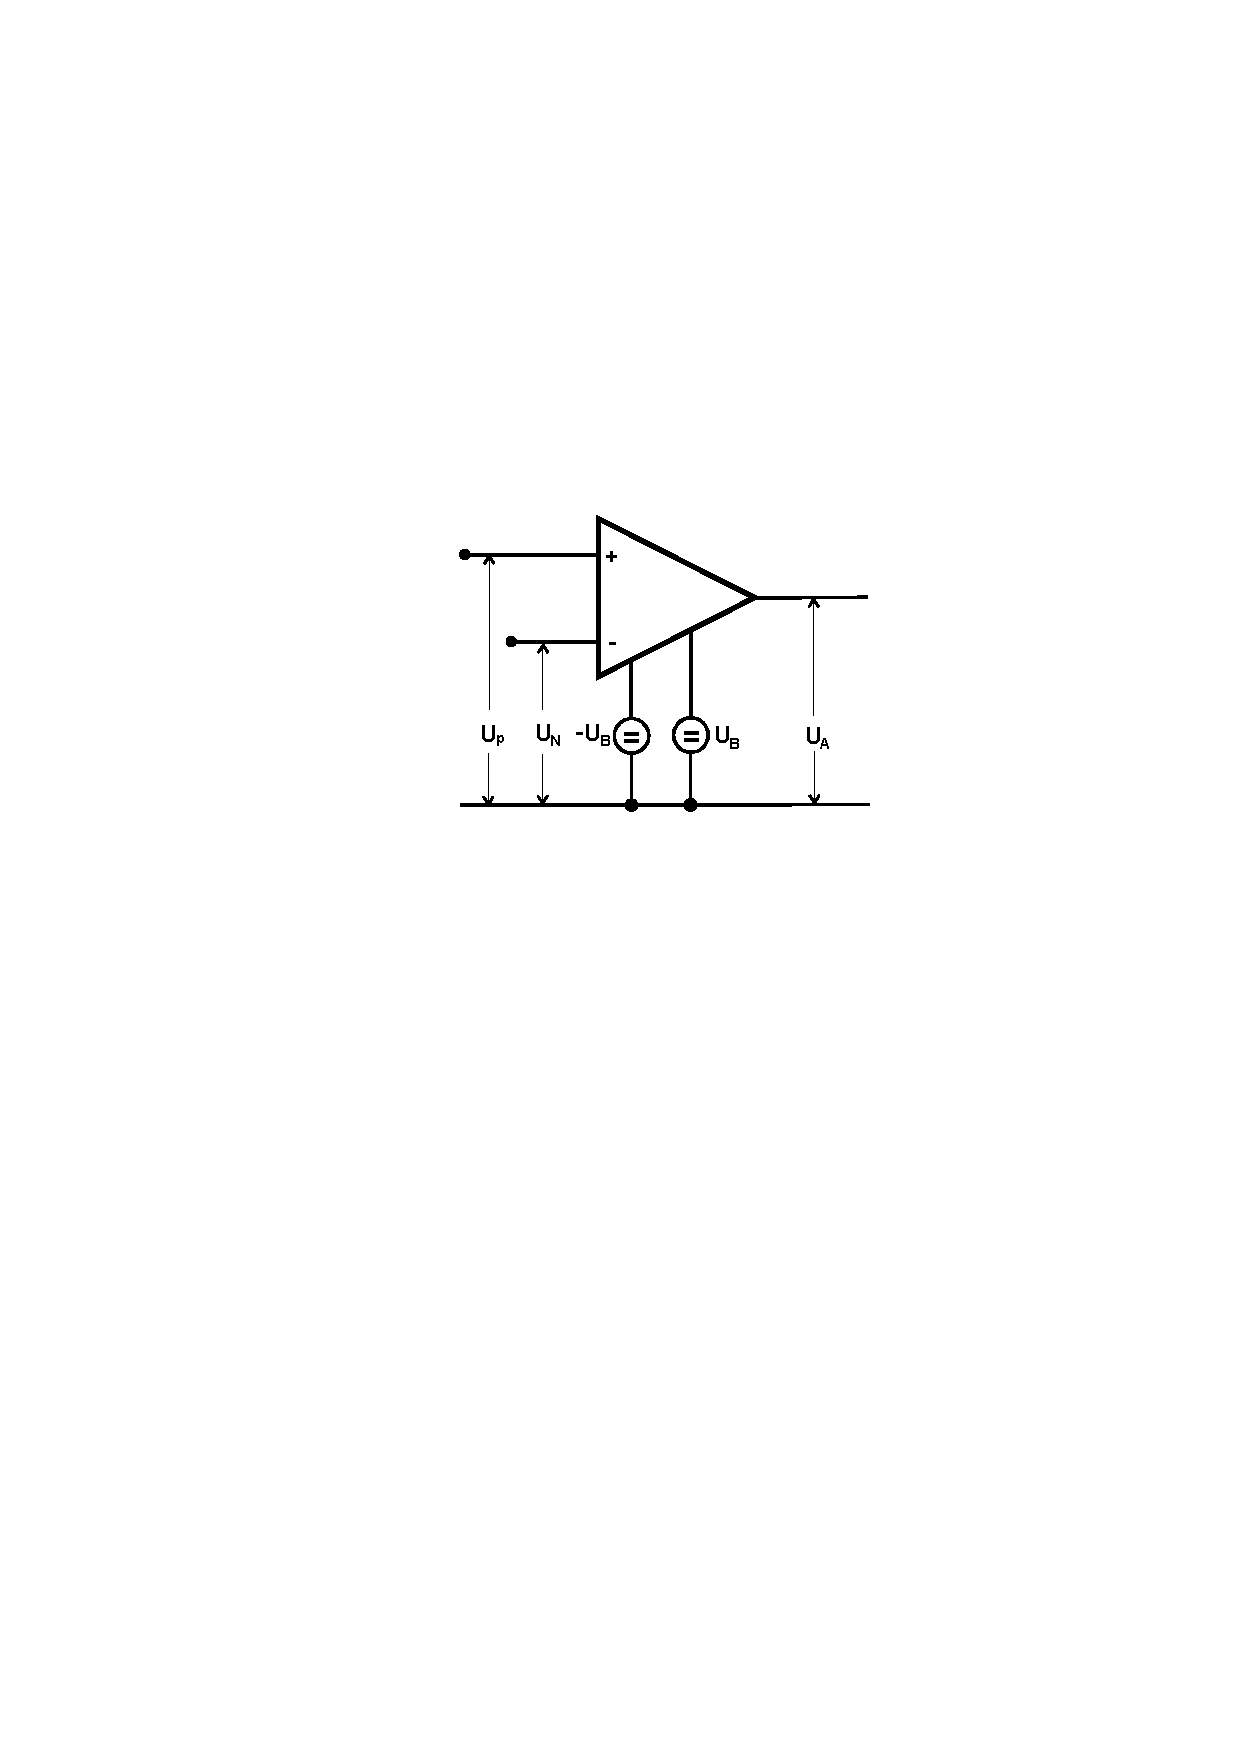
\includegraphics[width=0.5\linewidth]{img/op.pdf}
    \caption{
        Schaltbild eines Operationsverstärkers mit Ausgangsspannung
        $U_\text{A}$ und Eingangsspannungen $U_\text{p}$ und
        $U_\text{N}$ \cite{V51}.
    }
    \label{fig:op}
\end{figure}
Neben der meist frequenzabhängigen Leerlaufverstärkung $V$ besitzt der
Operationsverstärker weitere Kenngrößen, wie die Eingangswiderstände,
$r_\text{e,p}$ und $r_\text{e,N}$, sowie 
einen Ausgangswiderstand $r_\text{a}$.
Um Rechnungen zu Vereinfachen gilt für einen idealen Operationsverstärker
\begin{equation}
\label{eq:id-verstärker}
    V = \infty\,,\qquad r_\text{e} = \infty\,,\qquad r_\text{a} = 0\,.
\end{equation}

Im Gegensatz dazu müssen zur theoretischen Beschreibung eines realen
Operationsverstärkers zusätzliche Kenngrößen in Betracht gezogen werden.

Die Gleichtaktverstärkung
\begin{equation}
\label{eq:gleichtaktverstärkung}
    V_\text{Gl} = \frac{\Delta U_\text{A}}{\Delta U_\text{Gl}}
\end{equation}
berücksichtigt geringe Asymmetrien der beiden Vertärkungskanäle.
Dabei bezeichnen $\Delta U_\text{A}$ die Differenz der Ausgangsspannung zu
\num{0} und $\Delta U_\text{Gl}$ den Unterschied der -- eigentlich gleichen --
Eingangsspannungen.

Die auf Grund endlicher Eingangswiderstände $r_\text{e}$ auftretenden
Eingangsströme werden mit $I_\text{p}$ und $I_\text{N}$, deren
Mittelwert,
\begin{equation}
\label{eq:eingangsruhestrom}
    I_\text{B} = \frac{1}{2}\left(I_\text{p} + I_\text{N}\right)\,,
\end{equation}
als Eingangsruhestrom und die Differenz
\begin{equation}
\label{eq:offsetstrom}
    I_\text{B} = \frac{1}{2}\left(I_\text{p} + I_\text{N}\right)\,,
\end{equation}
als Offsetstrom bezeichnet.
Ähnlich zum Offsetstrom, verschwindet auch die Spannung häufig nicht.
Für die Offsetspannung $U_0$ gilt daher bei $U_\text{A} = 0$
\begin{equation}
\label{eq:offsetspannung}
    U_0 = U_\text{t} - U_\text{N}\,.
\end{equation}
Sie ist abhängig von Temperatur, Zeit und Betriebsspannungen. Die totale
Ableitung wird mit Offsetspannungsdrift bezeichnet.


\section{Schaltungsbeispiele}
\label{sec:schaltungsbeispiele}
Im Folgenden werden einige Schaltbeispiele für Operationsverstärker
dargestellt. Das Verhalten des Verstärkers hängt dabei meist nur von der
äußeren Schaltung ab und kann damit als annähernd ideal angenommen werden.

\subsection{Arten von Operationsverstärkern}

\subsubsection{Rückgekoppelter Linearverstärker}
\label{subsubsec:rueck-linearverstärker}
Der relativ kleine Arbeitsbereich des Operationsverstärkers ist in der
Anwendung oft nicht praktikabel. Um diesen Bereich zu verbreitern, wird die
Verstärkung reduziert, indem ein Teil der Ausgangsspannung auf den
invertierenden Eingang gegeben wird.
Der Anteil der zurückgeführten Spannung kann dabei mit Hilfe der Widerstände
$R_1$ und $R_\text{N}$ bestimmt werden, die in Abbildung \ref{fig:linear}
dargestellt sind.
\begin{figure}
    \centering
    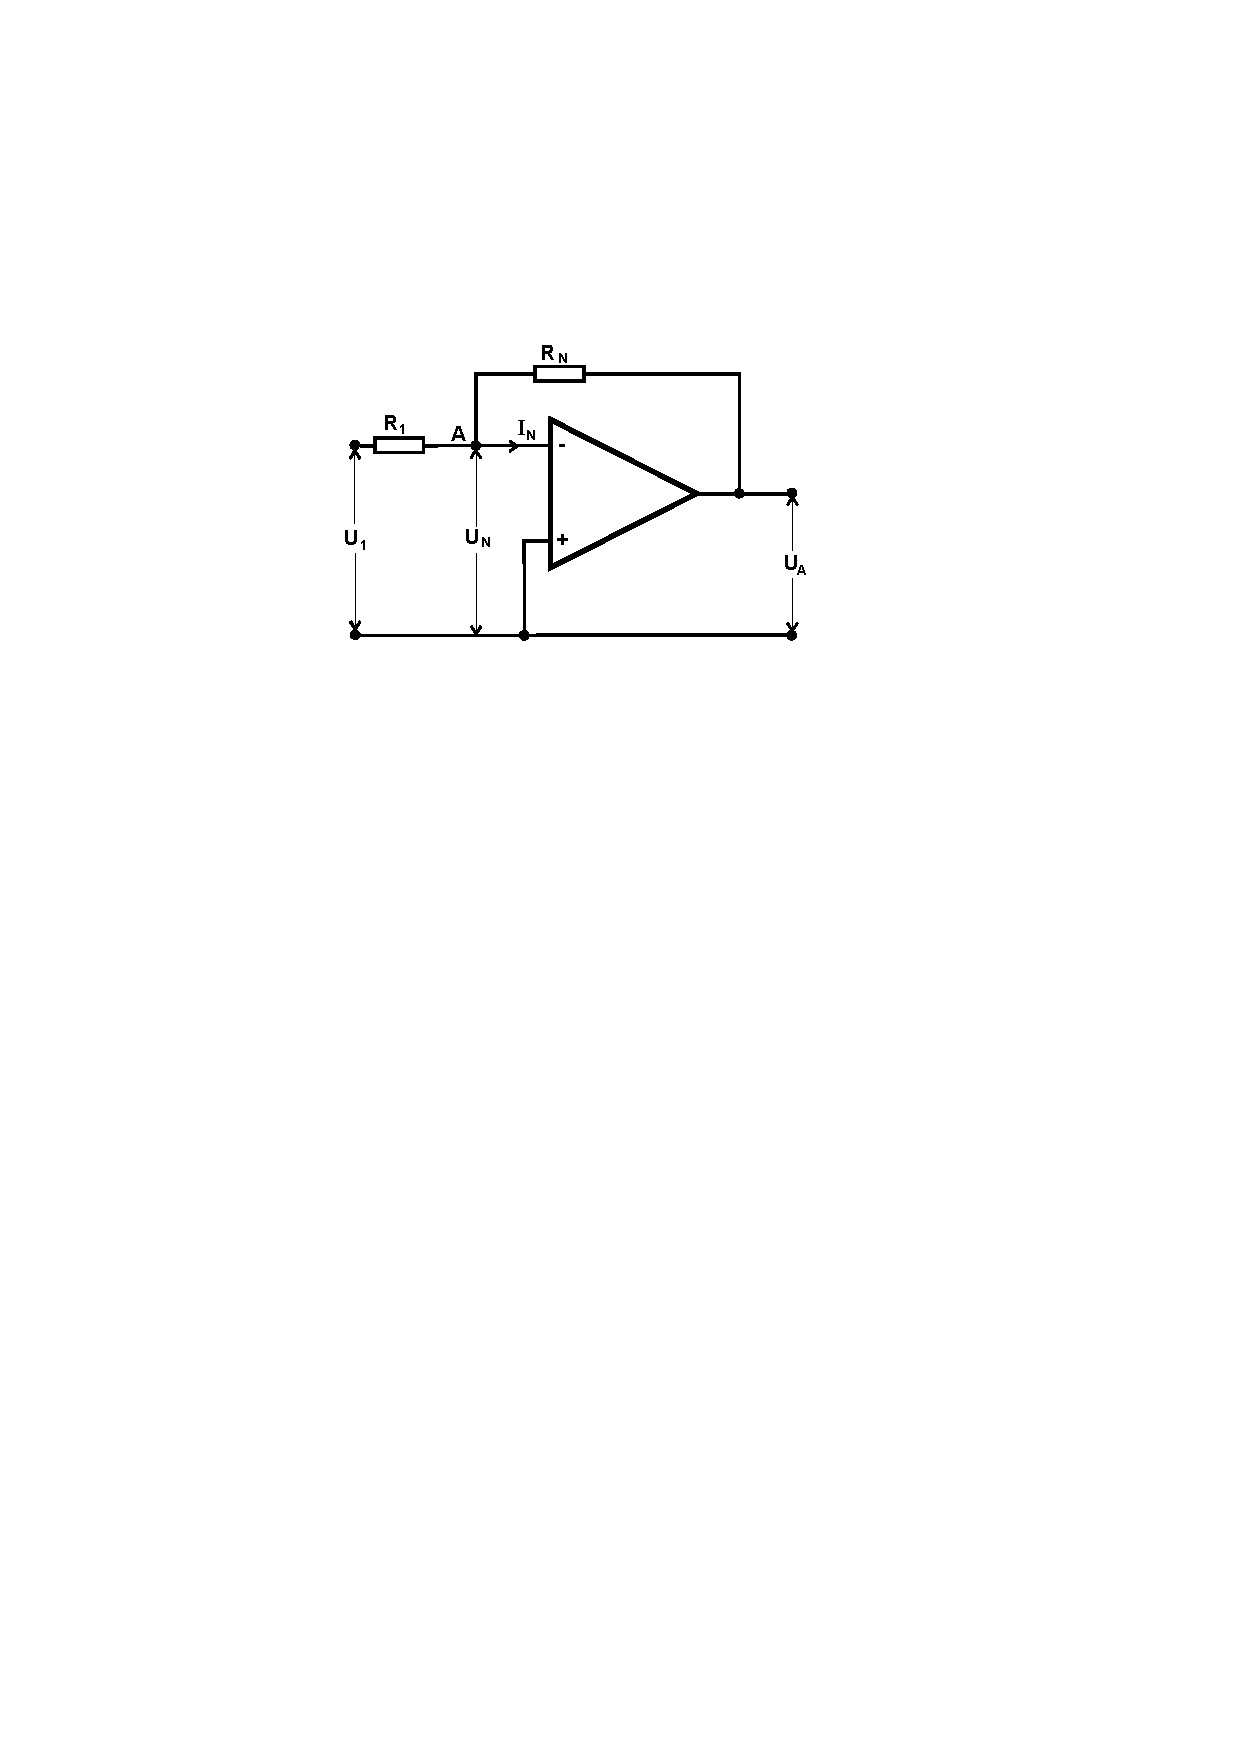
\includegraphics[width=0.5\linewidth]{img/linearverstaerker.pdf}
    \caption{Rückgekoppelter Linearverstärker \cite{V51}.}
    \label{fig:linear}
\end{figure}
Für den Fall $R_\text{N}/R_1 \ll V$
lässt sich zeigen, dass die Verstärkung $V^\prime$ nur noch vom Verhältnis
dieser beiden Widerstände abhängt.
Der Geringe Eingangswiderstand $r_\text{e} \approx R_1$ wirkt sich bei
hochohmigen Spannungsquellen möglicherweise nachteilig aus. Im nächsten
Abschnitt wird daher ein Linearverstärker vorgestellt, der diesen Nachteil
umgeht.

\subsubsection{Elektrometerverstärker}
\label{subsubsec:elektrometerverstärker}
Wie in Abbildung \ref{fig:elektrometer} deutlich wird, wird auch bei diesem
Verstärker ein Teil der Ausgangsspannung $U_\text{A}$ zum gegengekoppelten
Eingang zurückgeführt. Dabei sind die Widerstände $R_1$ und $R_\text{N}$ auf
eine andere Art und Weise verschaltet, sodass der Eingangswiderstand in der
Größenordnung des Gleichtakteingangwiderstandes
($r_\text{Gl} \approx \SI{10}{\giga\ohm}$) liegt, hier tritt das eventuelle
Problem des zu geringen Eingangswiderstandes als nicht auf.
Störend bei dieser Schaltung kann sich jedoch ein Eingangsruhestrom
$I_\text{B}$.
Die Verstärkung $V^\prime$ des Elektrometerverstärkers beträgt
\begin{equation*}
    V^\prime = \frac{U_\text{A}}{U_1} = \frac{R_\text{N} + R_1}{R_1}\,.
\end{equation*}
\begin{figure}
    \centering
    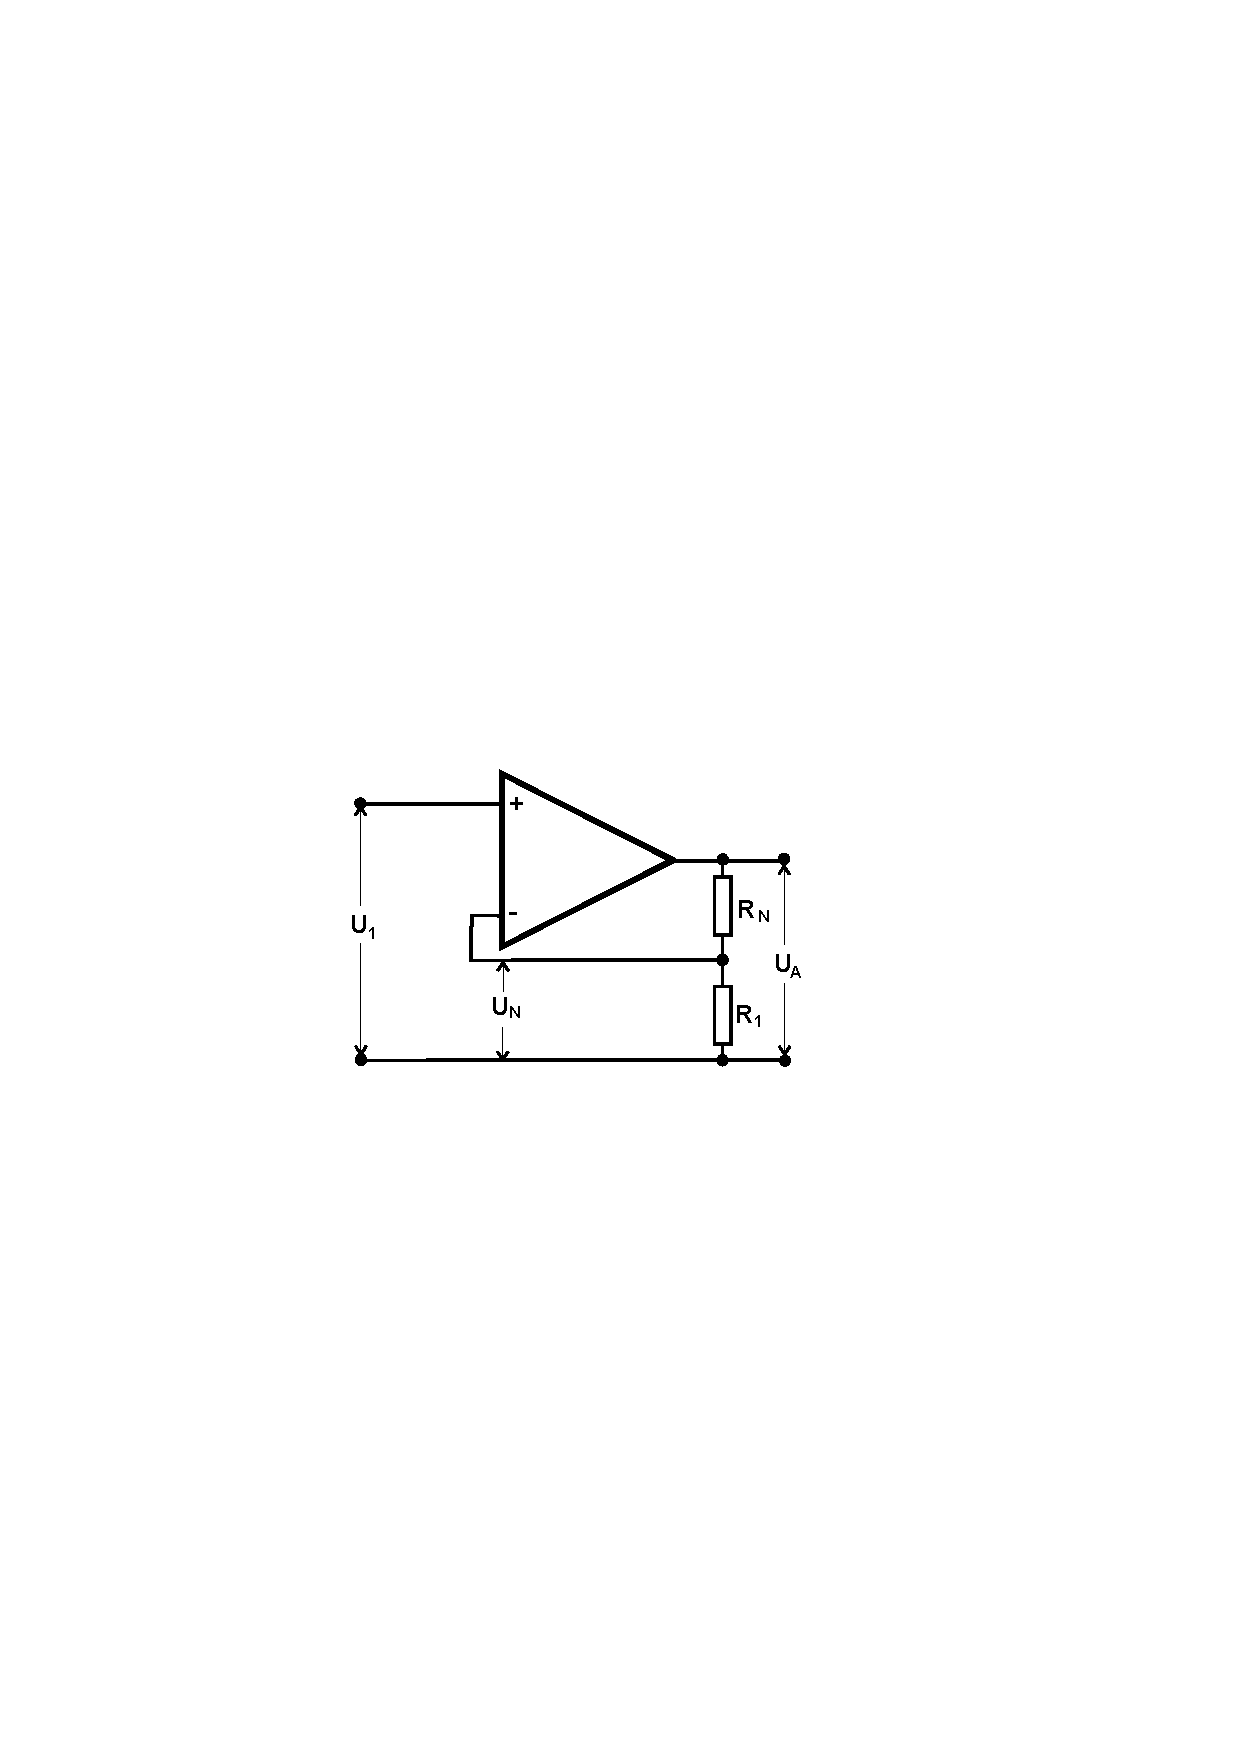
\includegraphics[width=0.5\linewidth]{img/elektrometer.pdf}
    \caption{Schaltbild eines Elektrometerverstärkers \cite{V51}.}
    \label{fig:elektrometer}
\end{figure}

\subsubsection{OP mit geringem Eingangswiderstand $R_\text{e}$ (Ampèremeter)}
\label{subsubsec:amperemeter}
Im Gegensatz zum grossen Eingangswiderstand $R_\text{e}$ eines 
Elektrometerverstärkers lässt sich, wie in Abbildung
\ref{fig:amperemeter} dargestellt, ein Linearverstärker mit 
besonders geringem Eingangswiderstand konstruieren.
Somit können zum Beispiel Ströme in einem Ampèremeter gemessen werden, wobei
der dazu nötige Spannungsabfall $\Delta U$ besonders gering ist.
\begin{figure}
    \centering
    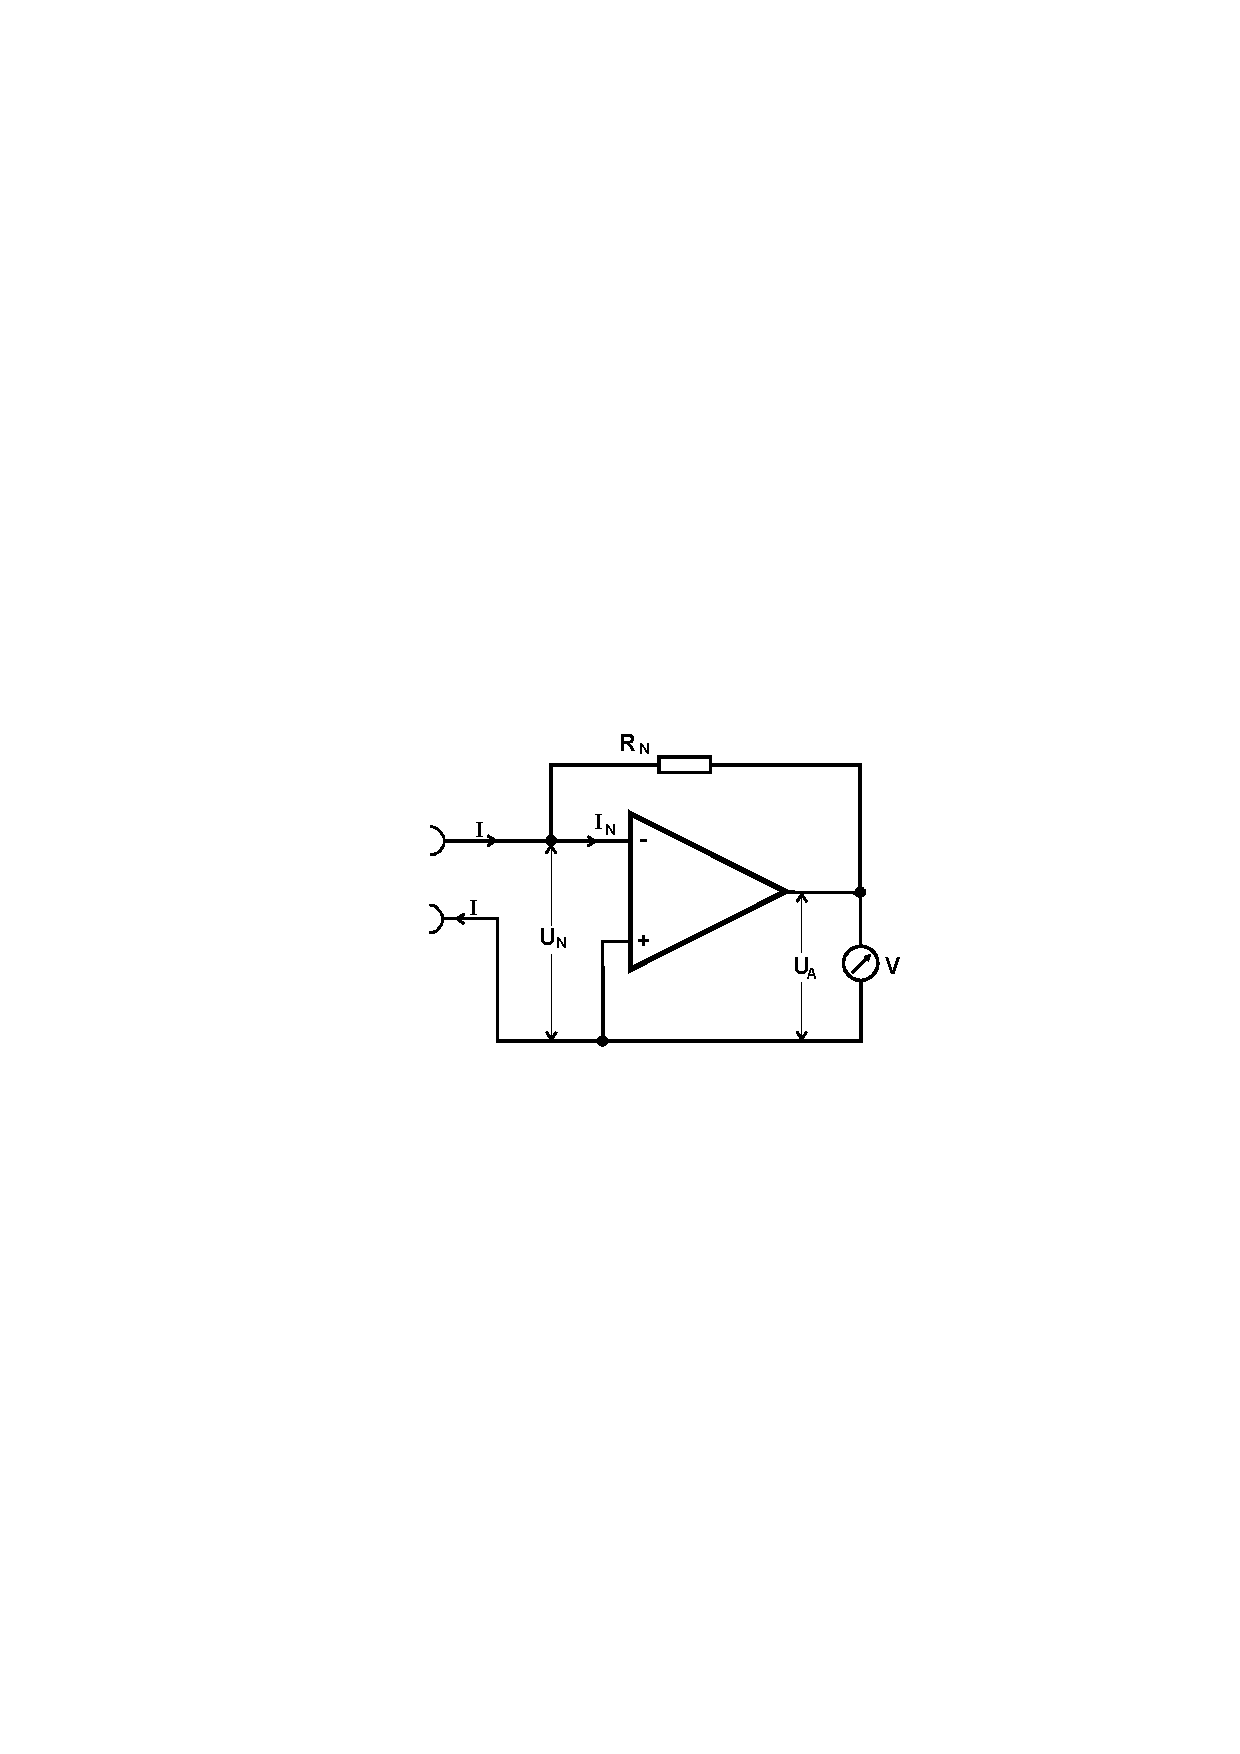
\includegraphics[width=0.5\linewidth]{img/amperemeter.pdf}
    \caption{Schaltbild eines Elektrometerverstärkers \cite{V51}.}
    \label{fig:amperemeter}
\end{figure}

\subsection{Umkehr-Integrator und -Differentiator}
\label{subsec:integrator}
Mit Hilfe eines zusätzlichen Kondensators mit Kapazität $C$ in der Schaltung
eines Linearverstärkers lässt sich entweder ein Integrations- oder eine
Differentiationsglied bauen.
Für die Ausgangsspannungen $U_\text{A,I}$ des Integrators und $U_\text{A,D}$
des Differentiators gilt dann
\begin{align*}
    U_\text{A,I} &= - \frac{1}{RC} \int U_1\!(t) \mathup{d}t\,,\\
    \text{und} \qquad U_\text{A,D} &= - RC \frac{\mathup{d}U_1}{\mathup{d}t}\,,
\end{align*}
wobei $R$ den Widerstand bezeichnet und Integrator und Differentiator sich
nur durch Position des Widerstandes und Kondensators unterscheiden.
Die entsprechenden Schaltungen sind in Abbildung \ref{fig:integrator}
dargestellt.
\begin{figure}
    \begin{subfigure}{.49\linewidth}
        \centering
        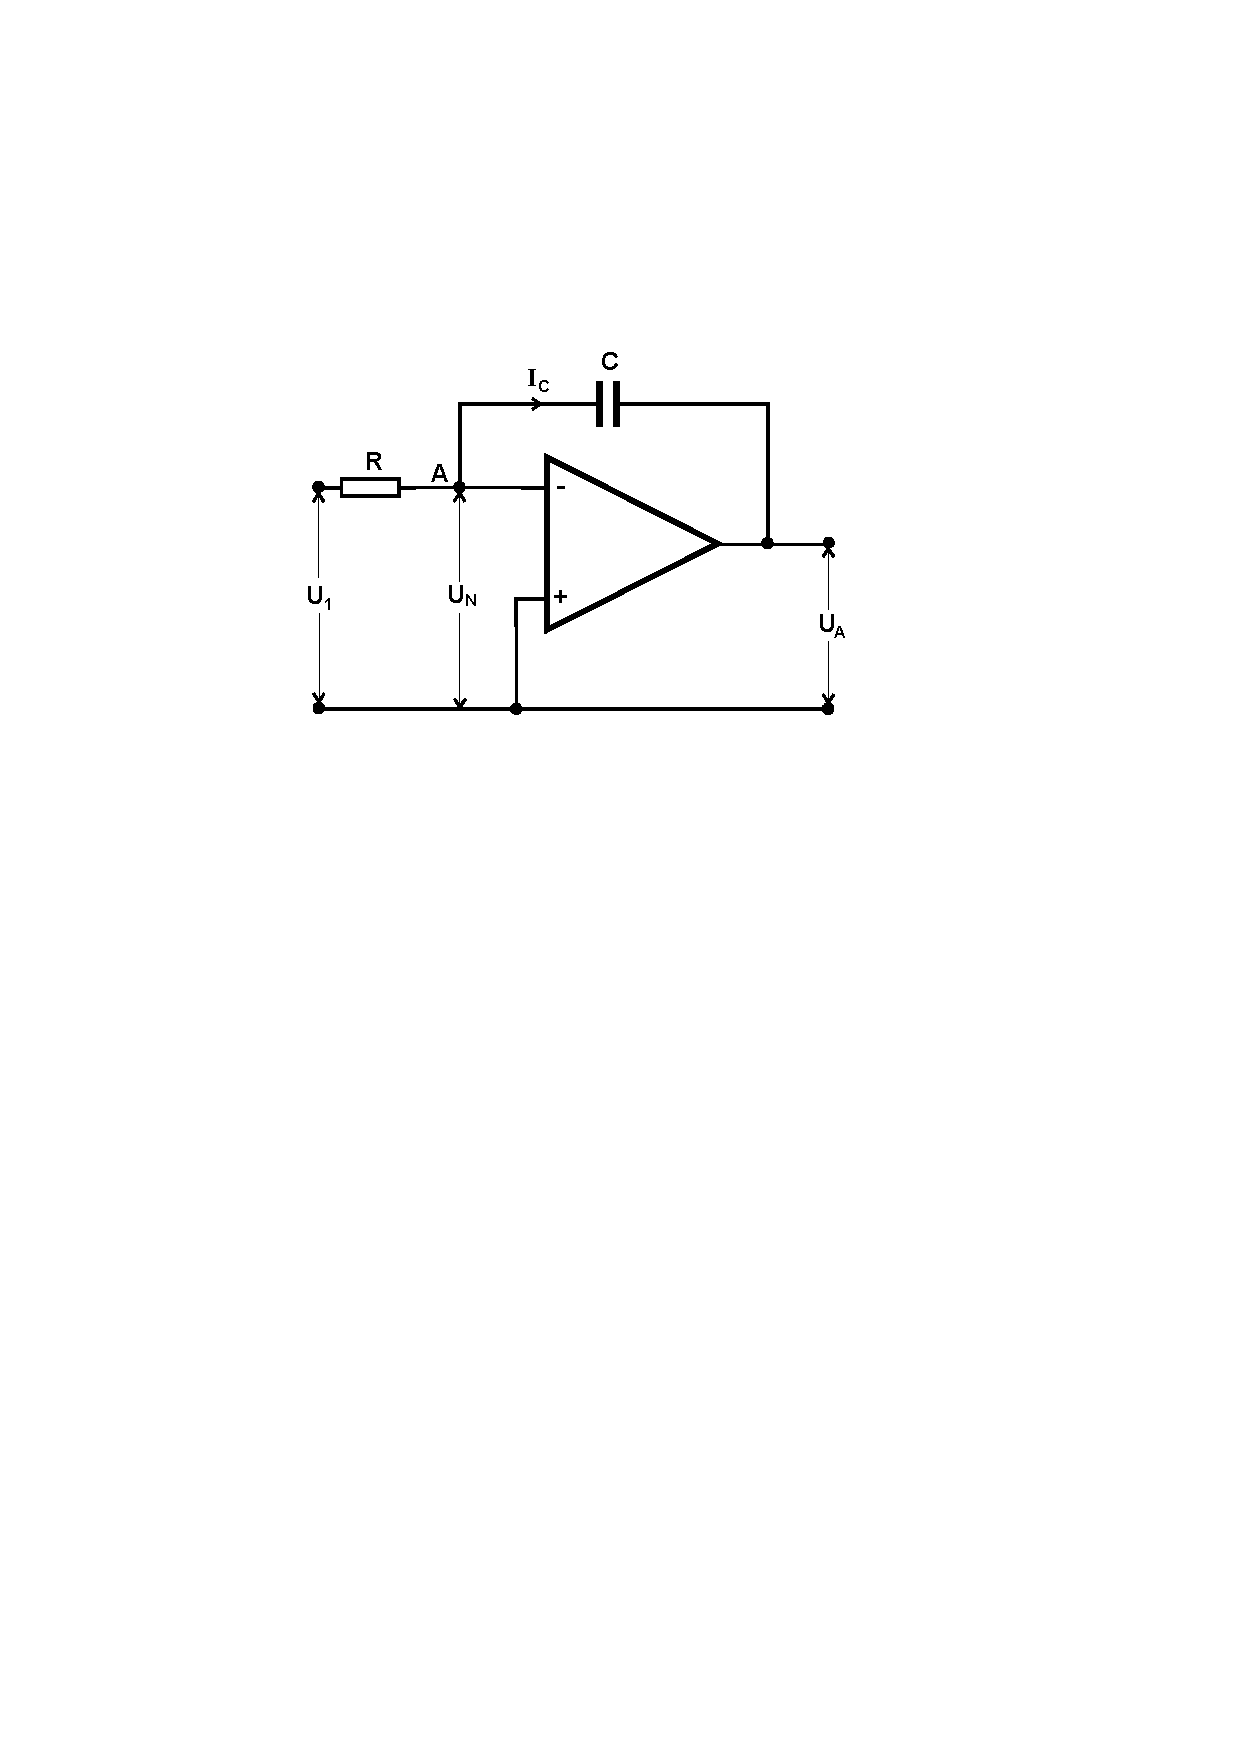
\includegraphics[width=1.0\linewidth]{img/integrator.pdf}
        \caption{Schaltbild eines Umkehr-Integrators \cite{V51}.}
        \label{fig:integrator-integrator}
    \end{subfigure}
    \begin{subfigure}{.49\linewidth}
        \centering
        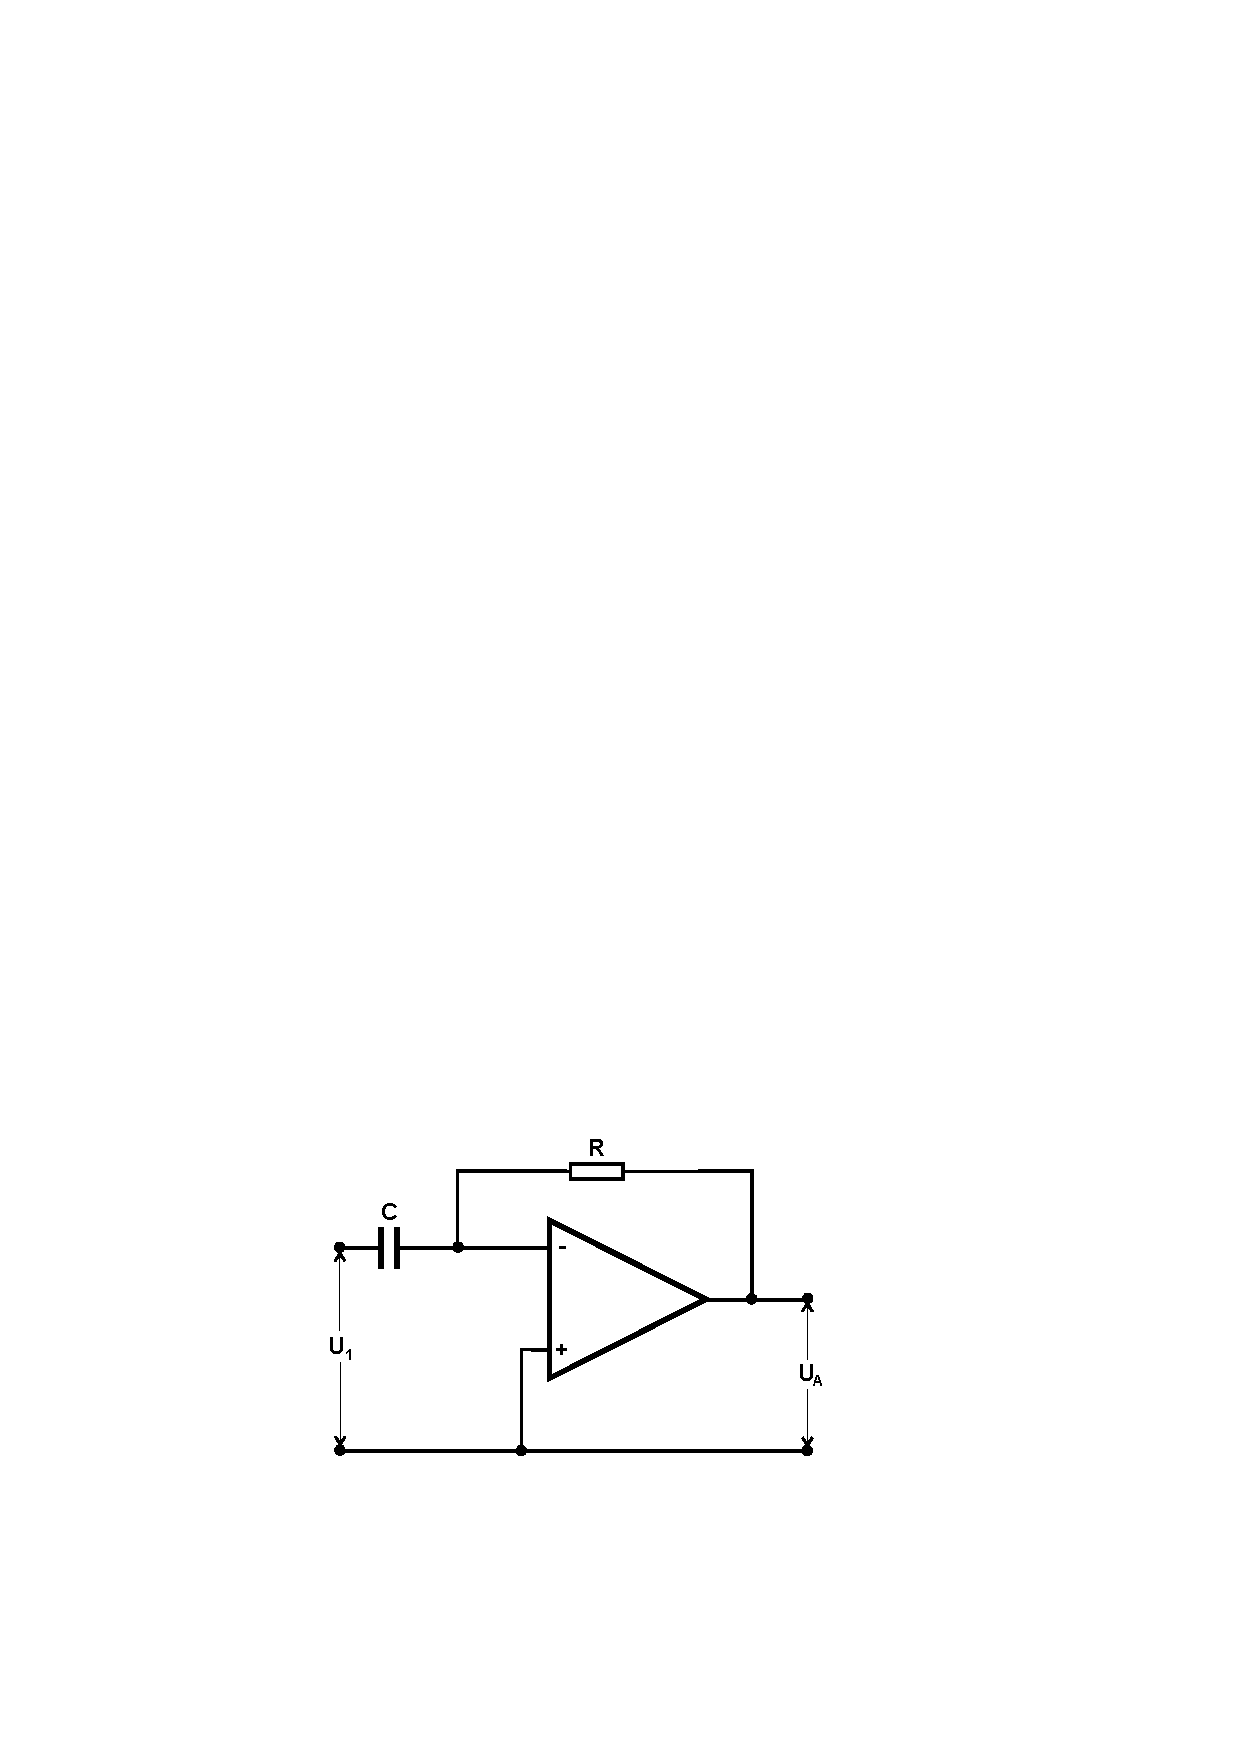
\includegraphics[width=1.0\linewidth]{img/differentiator.pdf}
        \caption{Schaltbild eines Umkehr-Differentiators \cite{V51}.}
        \label{fig:integrator-differentiator}
    \end{subfigure}
    \caption{Linearverstärker mit Kondensator.}
    \label{fig:integrator}
\end{figure}

\subsection{Logarithmierer und Exponentialgenerator}
\label{subsec:log_expo}
Neben Differential- und Integral-Operationen können auch Exponentierung nud
Logarithmierung mit Hilfe des Operationsverstärkers umgesetzt werden.
Dabei wird statt eines Kondensators eine Diode eingebaut.
Dabei gilt für die entsprechenden Ausgangssignale $U_\text{A,E}$ und 
$U_\text{A,L}$
\begin{align*}
    U_\text{A,L} &= R I \exp\left(\frac{e_0}{k_\text{B}T} U_\text{e}\right)\,,\\
    \text{und} \qquad U_\text{A,E} &= \frac{k_\text{B}T}{e_0}\ln \frac{U_\text{e}}{R I}\,,
\end{align*}
mit der absoluten Temperatur $T$, der Boltzmannkonstante $k_\text{B}$ und
der Elementarladung $e_0$. Abbildung \ref{fig:log_expo} zeigt die Schaltungen.
\begin{figure}
    \begin{subfigure}{.49\linewidth}
        \centering
        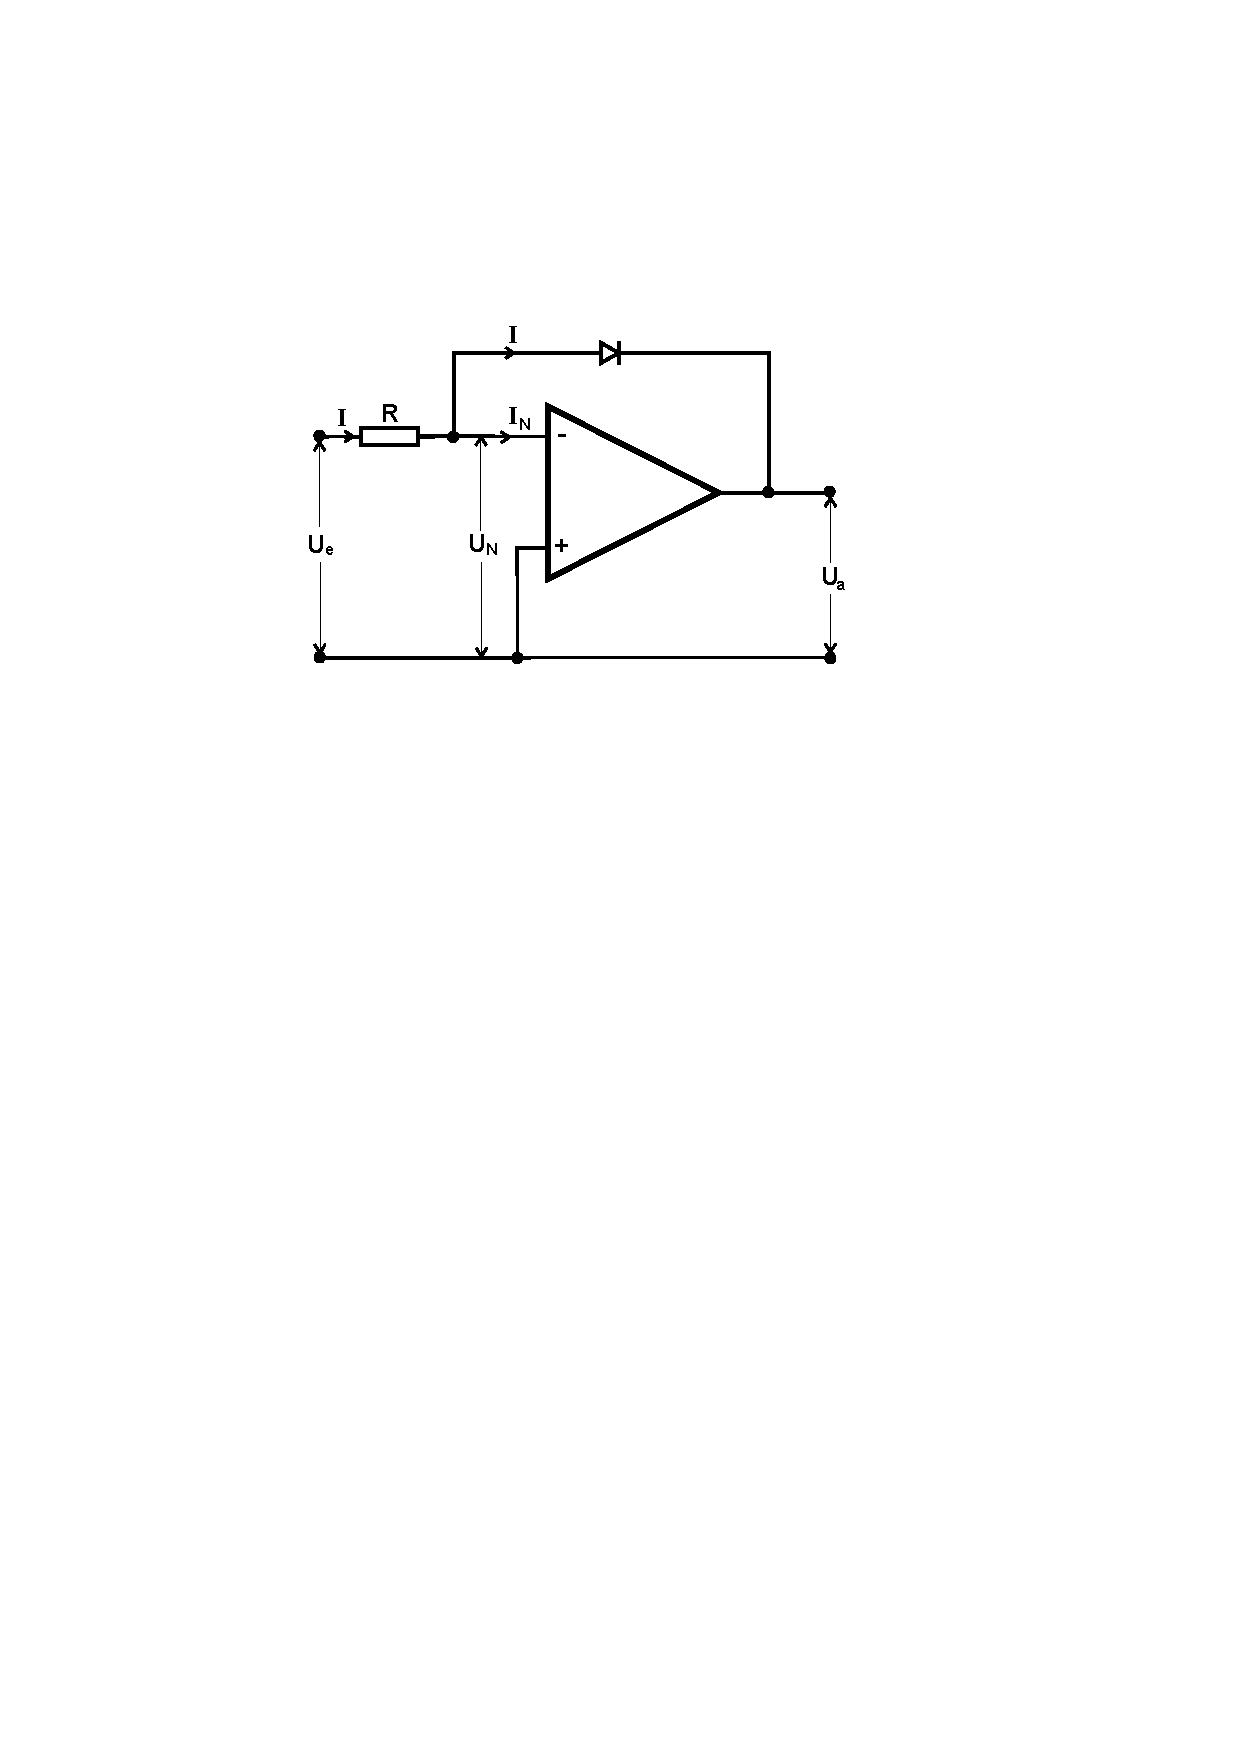
\includegraphics[width=1.0\linewidth]{img/log.pdf}
        \caption{Schaltbild eines Logarithmierers \cite{V51}.}
        \label{fig:log}
    \end{subfigure}
    \begin{subfigure}{.49\linewidth}
        \centering
        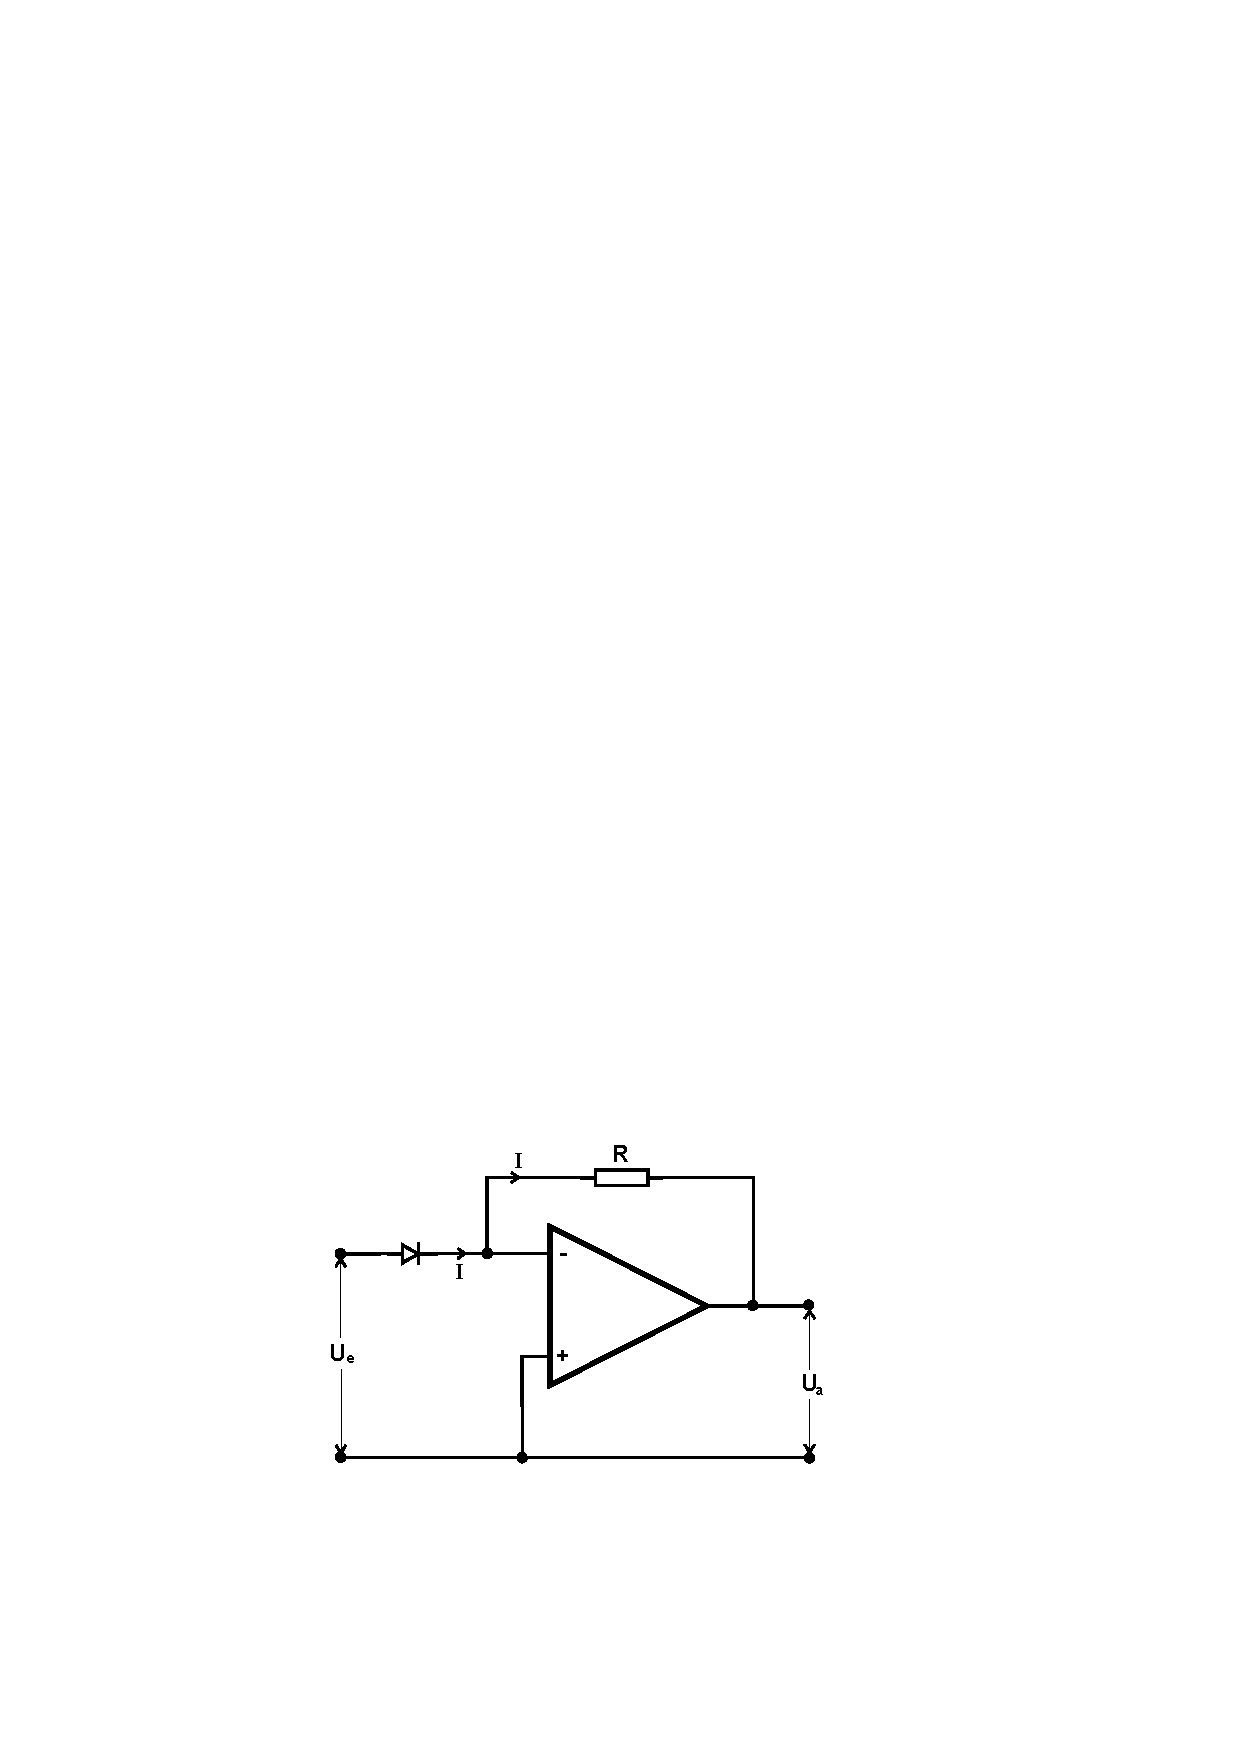
\includegraphics[width=1.0\linewidth]{img/expo.pdf}
        \caption{Schaltbild eines Exponentialgenerators \cite{V51}.}
        \label{fig:expo}
    \end{subfigure}
    \caption{Linearverstärker mit Kondensator.}
    \label{fig:log_expo}
\end{figure}

\subsection{Schmitt-Trigger}
\label{subsec:schmitt_trigger}
Der Operationsverstärker kann als Schalter genutzt werden. Statt, wie bisher
einen Teil der Ausgangsspannung auf einen gegengekoppelten Eingang zu geben,
wird dieser Anteil auf einen mitgekoppelten (invertierenden) Eingang gegeben.
Damit wird das eigene Ausgangssignal verstärkt, bis der Operationsverstärker
in eine Sättigung läuft.
Dabei beträgt das Ausgangssignal $U_\text{A}$ gerade
\begin{align*}
    U_\text{A} = 
    \begin{cases}
        +U_\text{B} &: U_1 > \frac{R_1}{R_\text{P}}U_\text{B} \\
        -U_\text{B} &: U_1 < -\frac{R_1}{R_\text{P}}U_\text{B}\,,
    \end{cases}
\end{align*}
mit der Betriebsspannugn $U_\text{B}$.
Die entsprechende Schaltung ist in Abbildung \ref{fig:schmitt_trigger}
dargestellt.
\begin{figure}
    \centering
    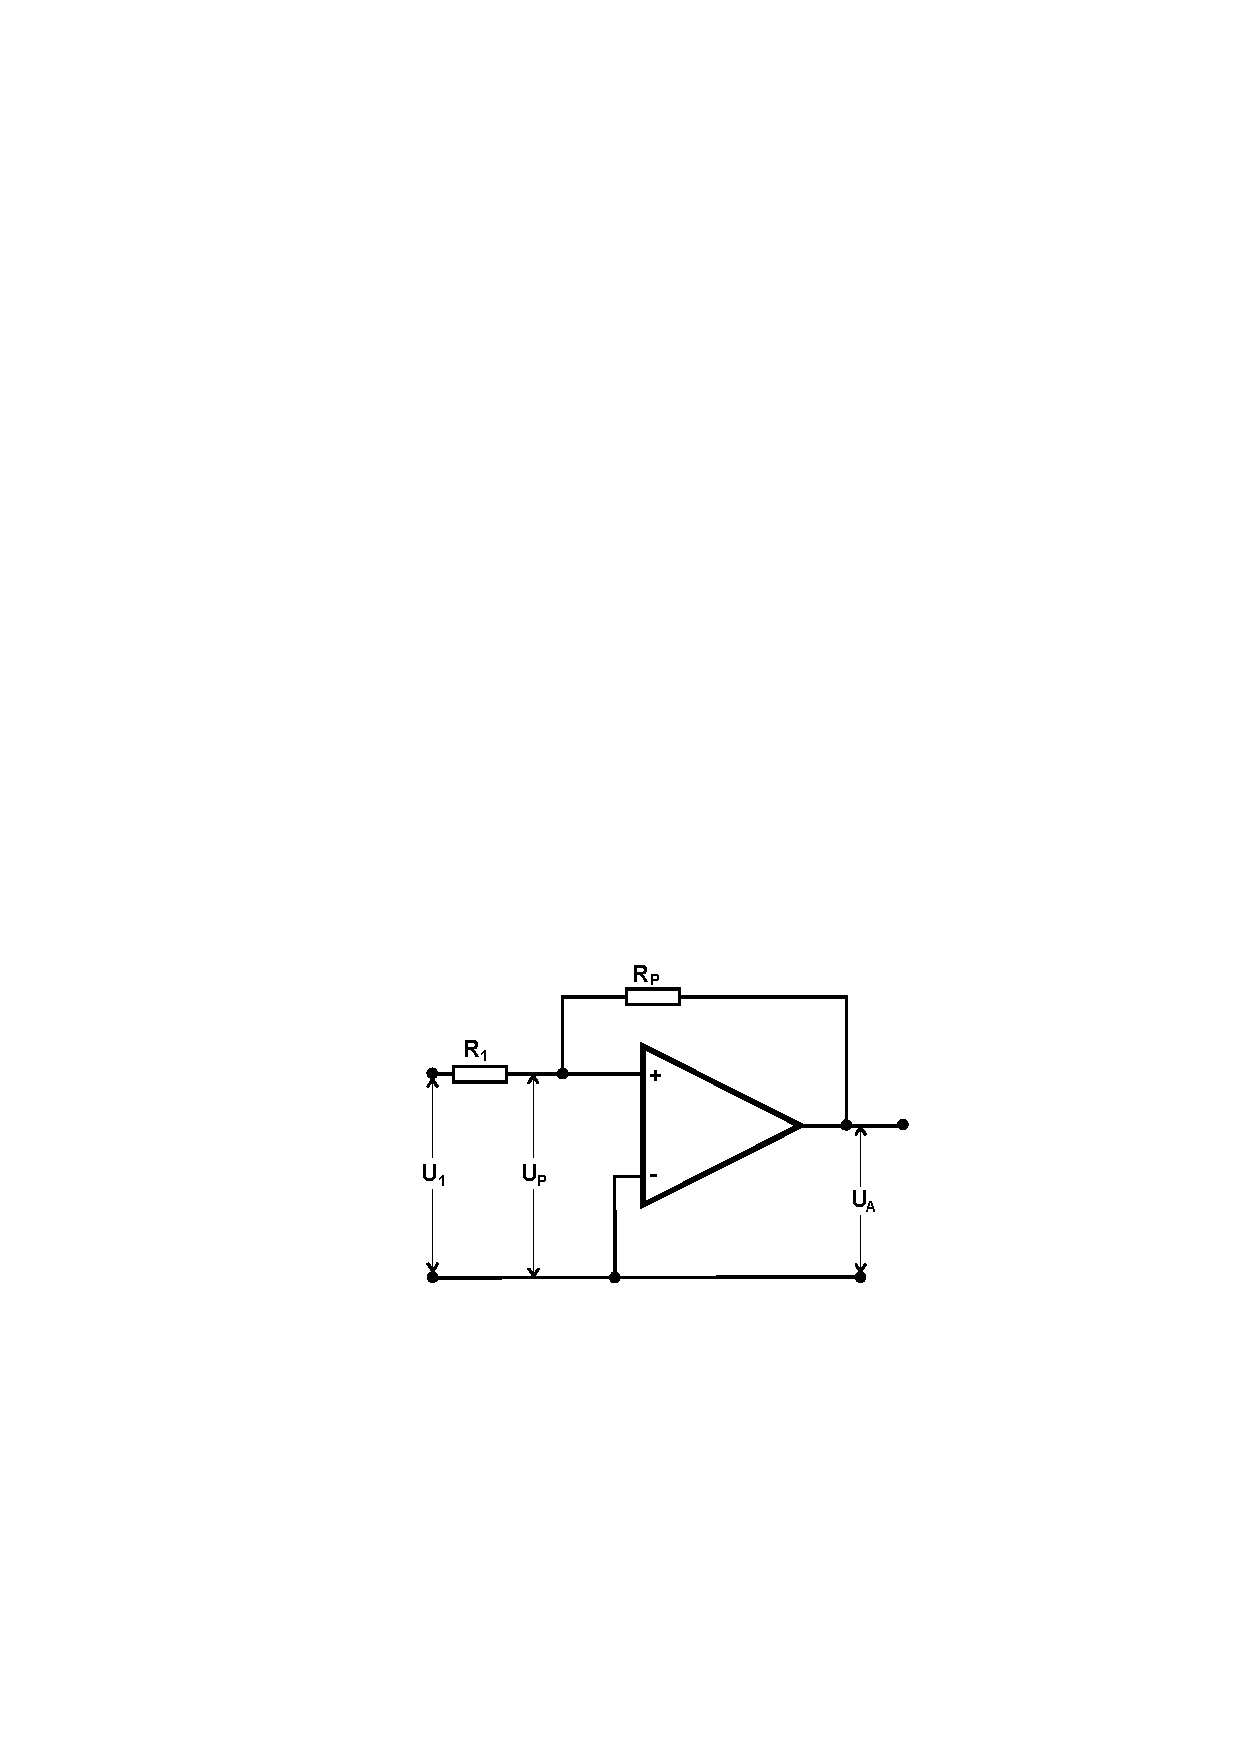
\includegraphics[width=0.5\linewidth]{img/schmitt_trigger.pdf}
    \caption{
        Schaltbild eines Operationsverstärker, der als Schmitt-Trigger
        genutzt wird.
    }
    \label{fig:schmitt_trigger}
\end{figure}

\subsection{Signalgenerator}
\label{subsec:signalgenerator}
Schließich können mit Hilfe eines Operationsverstärkers verschiedene
Signalspannungen erzeugt werden. Dazu wird jeweils eine Mehrzahl von OPs
miteinander verschaltet.

\subsubsection{Erzeugung von Dreieck- und Rechteckspannungen}
\label{subsubsec:dreieck}
Durch Kombination eines Schmitt-Triggers mit einem Integrationsglied
lassen sich Dreiecks- und Rechtecksspannungen erzeugen. Damit wird die
Integration genutzt, um den Schmitt-Trigger zu schalten und somit das
Vorzeichen des Signals zu ändern. Je nach Ausgang der in Abbildung
\ref{fig:dreieck} dargestellten Schaltung erhält man die gewünschte
Spannungsform.
\begin{figure}
    \centering
    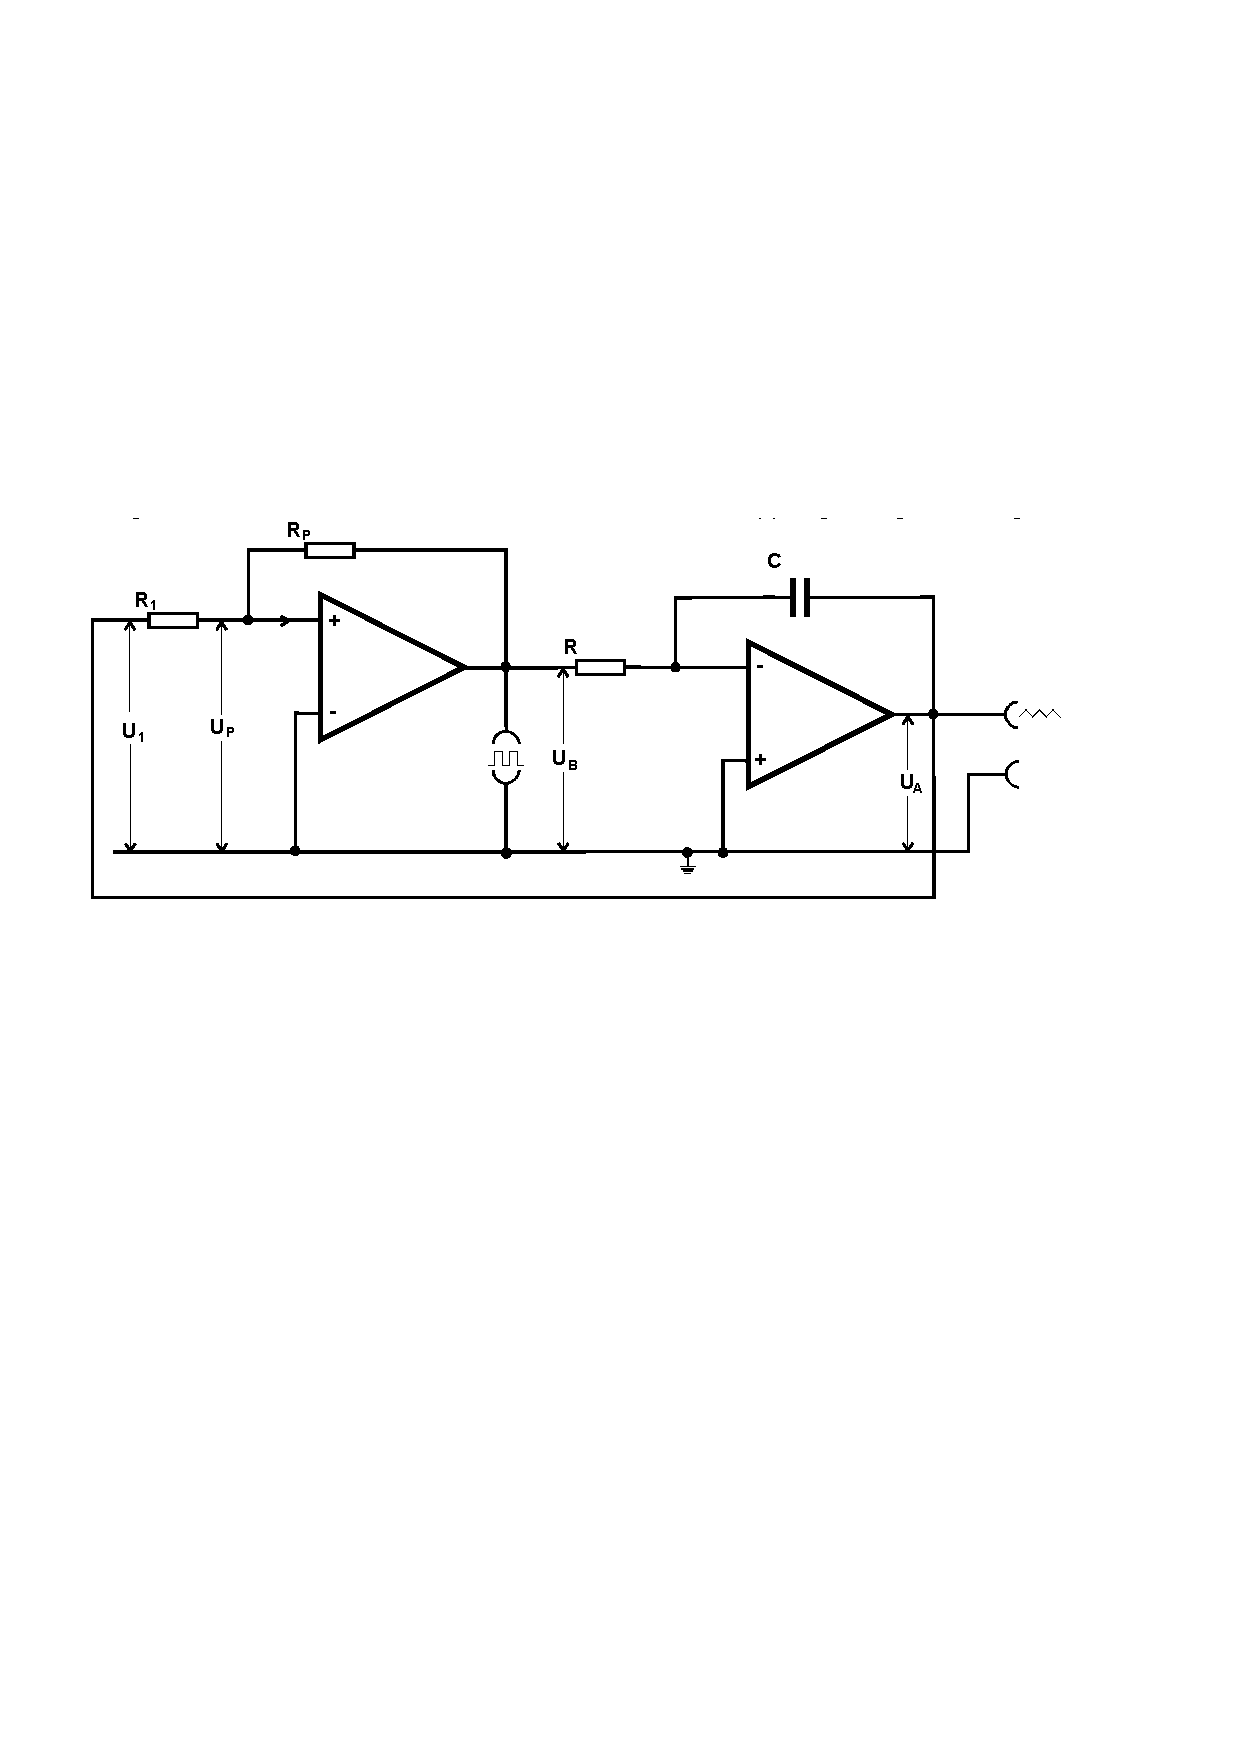
\includegraphics[width=0.9\linewidth]{img/dreieck.pdf}
    \caption{
        Schaltbild zur Erzeugung von Dreieck- und Recheckspannungen:
        Es wird ein OP als Integrationsglied mit einem Schmitt-Trigger
        verschaltet \cite{V51}.
    }
    \label{fig:dreieck}
\end{figure}

\subsubsection{Erzeugung von Sinusschwingungen}
\label{subsubsec:sinusschwingungen}
Durch Kombination zweier Integratoren mit einem Umkehrverstärker lassen sich
gedämpfte Sinusschwingungen erzeugen.
Die Schaltung kann durch eine Differetialgleichung 2. Ordung beschrieben
werden und liefert die Lösung
\begin{equation*}
    U_\text{A}(t) = U_0 \exp\!\left( \frac{\eta t}{\num{20} RC} \right)
                        \sin\!\left( \frac{t}{RC} \right)\,.
\end{equation*}
Dabei ist $\num{-1} < \eta < \num{1}$ durch das Potentiometer $P$ einzustellen.
Die Schwingungsdauer beträgt dabei $T = 2\pi RC$, die Abklingzeit
$\tau = 20 RC / |\eta|$. Damit sollte die Amplitude für $\eta = \num{0}$
konstant bleiben.
Das Schaltbild zu einem Sinusgenerator ist in Abbildung \ref{fig:sinus}
dargestellt
\begin{figure}
    \centering
    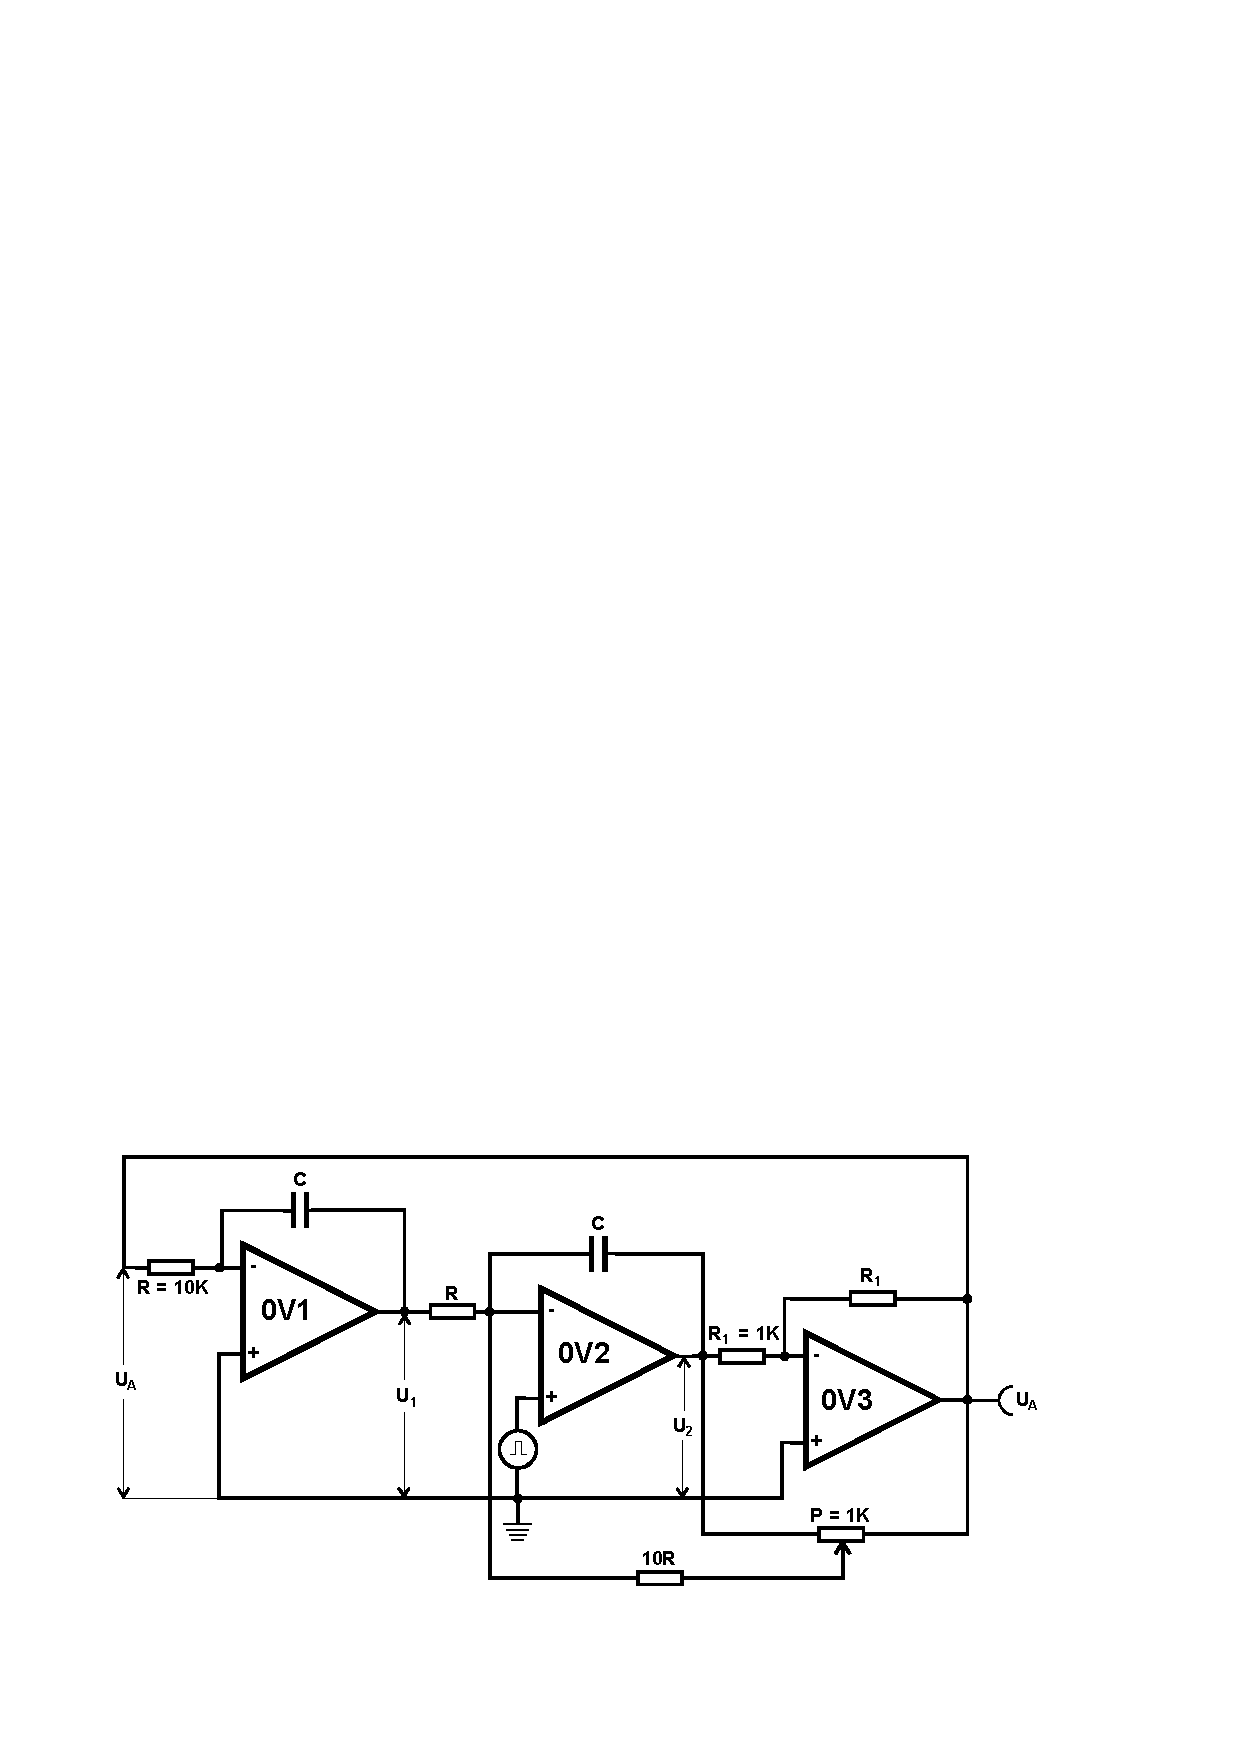
\includegraphics[width=0.9\linewidth]{img/sinus.pdf}
    \caption{
        Schaltbild eines Sinusgenerators. Es werden zwei Integrationsglieder
        und ein Umkehrverstärker verbaut \cite{V51}.
    }
    \label{fig:sinus}
\end{figure}

\clearpage
